\chapter{Cosmological Inference}
\label{ch:cosmological_inference}

Cosmological parameters are inferred from noisy, incomplete, and heterogeneous data (CMB, large-scale structure, distance ladders, ...). This chapter summarizes the statistics used throughout modern observational cosmology, with emphasis on Bayesian inference, practical sampling methods, checks on fit quality, and common pitfalls when comparing models and data sets.

\section{Bayesian and frequentist statistics}

In cosmology we have two complementary ways of attaching uncertainty to conclusions.

\begin{itemize}
    \item \textbf{Frequentist viewpoint:} \textit{Model is fixed, data are repeatable.} The model parameters are treated as fixed (though unknown) constants, and probability quantifies the variability of data under repeated sampling. Probability is defined as ``the number of times the event occurs over the total number of trials, in the limit of an infinite series of equiprobable repetitions.''

    \item \textbf{Bayesian viewpoint:} \textit{Data are fixed, model is repeatable.} The unknown model parameters are treated as \textit{random variables} with probability distributions, and statements about probability refer to the degree of belief we assign given the available information. Probability captures our uncertainty about parameters, not just random draws of data.
\end{itemize}

\begin{observationblock}[Repeatability]
        Real cosmological observations are not drawn from an ensemble of identical universes. This does not invalidate frequentist tools, but it explains why probability statements about \emph{parameters} are often phrased indirectly (confidence intervals, $p$-values) rather than as direct ``degrees of belief''.
\end{observationblock}

In practice, Bayesian methods dominate parameter estimation in cosmology because they combine heterogeneous experiments naturally (via hierarchical models), propagate nuisance parameters cleanly, and deliver interpretable uncertainty regions for physical quantities.

\begin{exampleblock}[$H_0 = (72 \pm 8)$~km\,s$^{-1}$\,Mpc$^{-1}$]
    \begin{itemize}
        \item \textcolor{red!80!black}{\textbf{Bayesian:}} The posterior distribution for $H_0$ has 68\% of its integral between 64 and 80 km/s/Mpc. The posterior can then be used as a prior in a new application of Bayes' theorem.
        \item \textcolor{blue!80!black}{\textbf{Frequentist:}} Performing the same procedure will cover the real value of $H_0$ within the limits 68\% of the time. But how do I repeat the same procedure if I only have one Universe?
    \end{itemize}
\end{exampleblock}

\begin{minipage}[t]{0.48\textwidth}
    \textbf{Bayesian workflow}
    \begin{itemize}
        \item Models give probabilities
        \item Inferences depend on both likelihood and prior (for parameters \emph{and} for models).
        \item Standard in CMB, weak lensing, BAO, and most Monte Carlo pipelines.
    \end{itemize}
\end{minipage}
\hfill
\begin{minipage}[t]{0.48\textwidth}
    \textbf{Frequentist workflow}
    \begin{itemize}
        \item Emphasis on likelihood-based estimators and calibrated coverage.
        \item No prior over parameters is required.
        \item Still common in particle physics (e.g.\ hypothesis tests with $p$-values).
    \end{itemize}
\end{minipage}

\subsubsection{Bayes' theorem}
\label{sec:bayes_theorem}

Let $d$ denote the observed data and $\theta$ the collection of parameters of a model $M$. Bayes' theorem relates the \textbf{posterior} density for the parameters to the \textbf{likelihood} of the data and the \textbf{prior} density over parameters:

\begin{definitionblock}[Bayes' theorem (parameter inference)]
    $$
    p(\theta \mid d, M)
    = \frac{P(d \mid \theta, M)\,P(\theta \mid M)}{P(d \mid M)}
    \qquad\text{equivalently}\qquad
    p(\theta \mid d, M) \propto P(d \mid \theta, M)\,P(\theta \mid M)
    $$
    where:
    \begin{itemize}
        \item $p(\theta \mid d, M)$ is the \textbf{posterior} (state of knowledge about parameters after the measurement);
        \item $P(d \mid \theta, M)$ is the \textbf{likelihood} ($\mathcal{L}$) (probability density assigned to the observed data for fixed $\theta$);
        \item $P(\theta \mid M)$ is the \textbf{prior} ($\pi$) (density encoding information before the experiment);
        \item $P(d \mid M) = \int P(d \mid \theta, M)\,P(\theta \mid M)\,\dd{\theta}$ is the \textbf{evidence} ($\mathcal{Z}$) (normalization constant).
    \end{itemize}
\end{definitionblock}

The evidence is a normalization constant for parameter estimation, but it becomes central when comparing different models $M_i$ with different dimensionalities or priors.

\section{Priors}
\label{sec:priors}

The prior $\pi(\theta \mid M)$ should summarize everything known about parameters \emph{before} incorporating the likelihood from the experiment at hand. That can include physical boundaries (e.g.\ $\Omega_m > 0$), stability of the theory, or results from previous experiments (hierarchical priors).

In regions where the likelihood is exactly zero, the prior is irrelevant for the posterior shape, but it still affects Bayesian model comparison.

Flat priors are widely used for location parameters, but ``flat'' is not reparameterization invariant. If $\psi = g(\theta)$ is an invertible transformation, conservation of probability requires
$$
\pi_\psi(\psi) = \pi_\theta(\theta)\,\left|\frac{\dd{\theta}}{\dd{\psi}}\right|.
$$
A prior uniform in $\theta$ generally induces a \emph{non-uniform} prior on $\psi$ unless $g$ is affine. This Jacobian factor is the algebraic reason why ``uninformative'' is a misnaming: any proper prior encodes a measure on parameter space.

\begin{figure}[H]
    \centering
    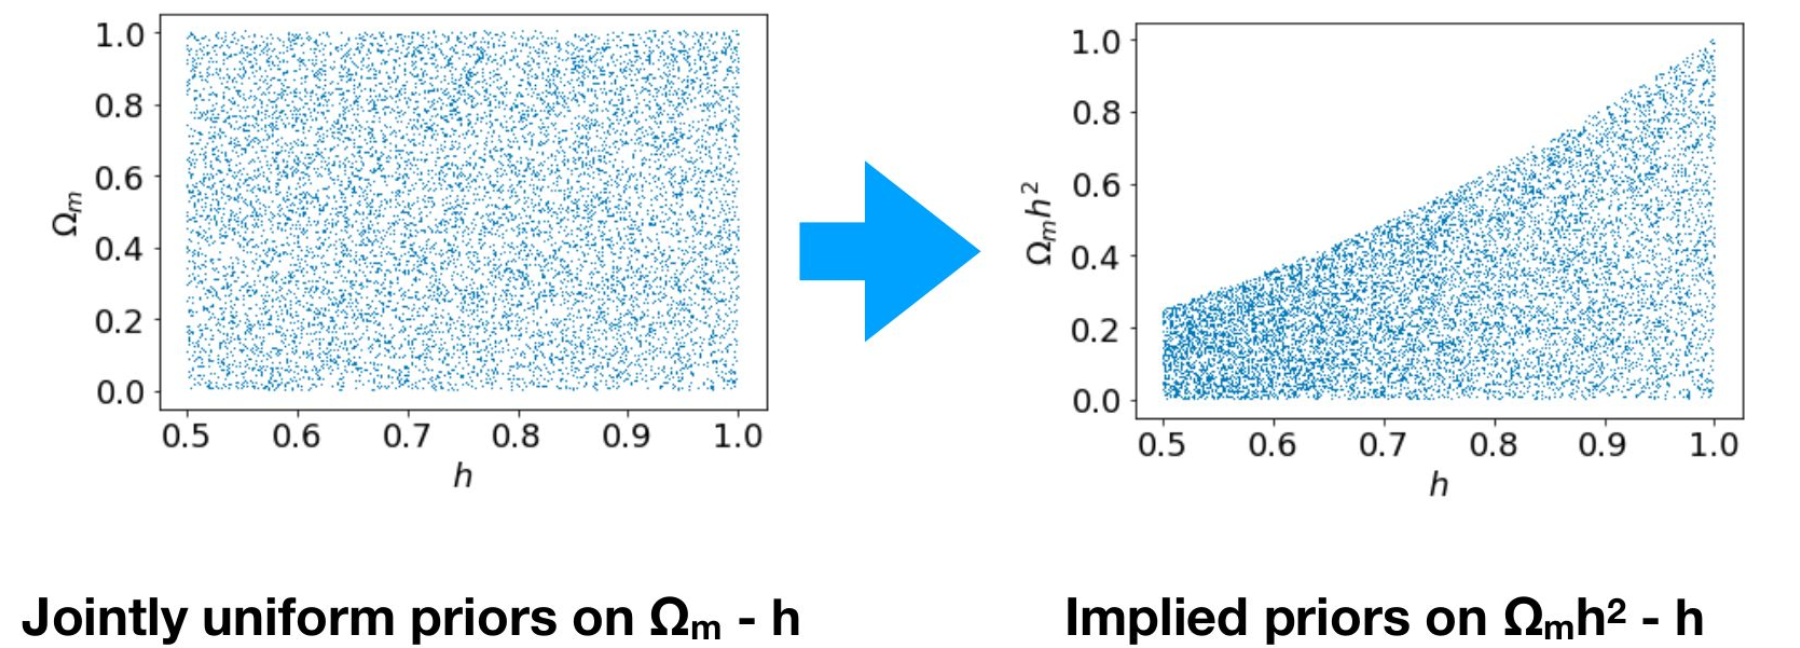
\includegraphics[width=0.9\textwidth]{assets/priors_ex.png}
\end{figure}

\subsubsection{Example: priors on dynamical dark energy}

Broad uniform priors on parametrizations such as the CPL pair $(w_0, w_a)$ allocate substantial prior mass to regions that are physically extreme or poorly constrained by the data. Posteriors and tensions can then shift noticeably when one instead uses priors motivated by scalar-field potentials (``hilltop'', ``exponential'', etc.), even when the likelihood is unchanged.

\begin{figure}[H]
    \centering
    \begin{minipage}{0.45\textwidth}
        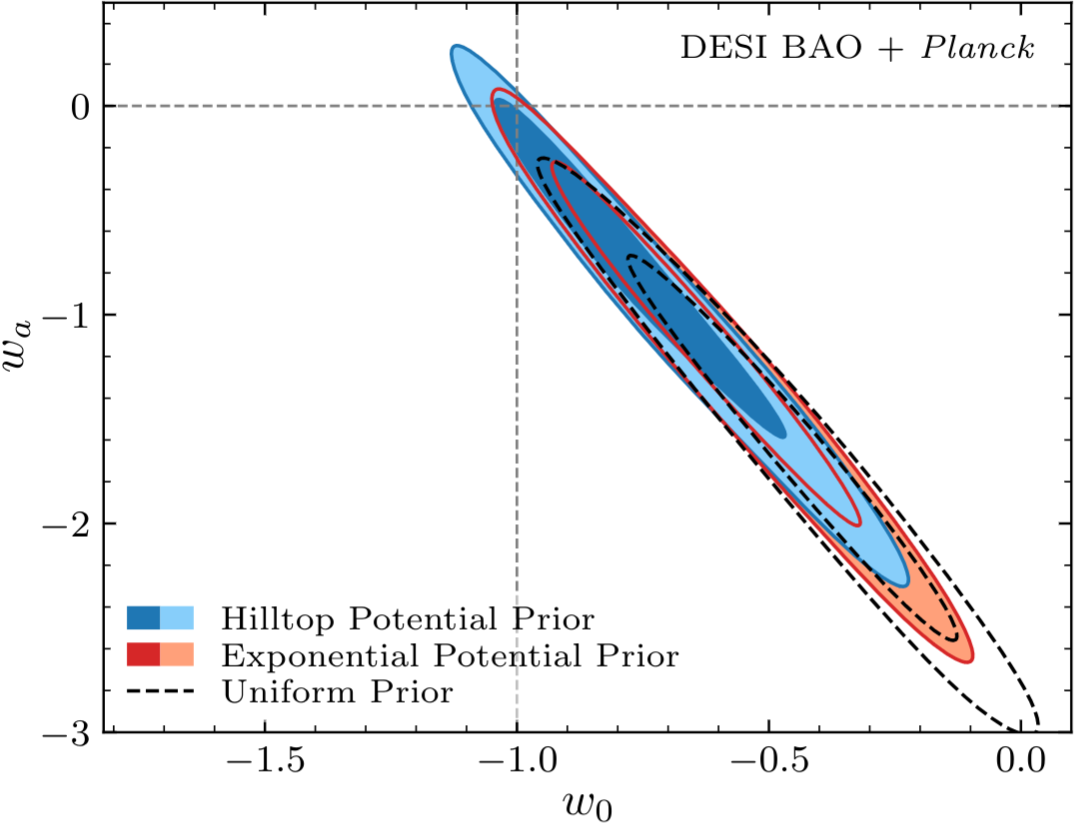
\includegraphics[width=\textwidth]{assets/priors.png}
    \end{minipage}%
    \hfill
    \begin{minipage}{0.5\textwidth}
        \captionof{figure}{Two-dimensional posteriors for $(w_0, w_a)$ at 68\% and 95\% credible levels (Planck PR4 + DESI DR2), illustrating prior dependence for evolving dark energy models. Gray dashed lines mark the $\Lambda$CDM point $(w_0, w_a) = (-1, 0)$. Theory-motivated priors (blue: hilltop; red: exponential) pull the distribution toward $\Lambda$CDM compared with a very broad uniform prior (black dashed). The lesson is operational: always document priors and, when possible, check sensitivity.}
        \label{fig:w0wa_priors}
    \end{minipage}
\end{figure}

\vspace{-2.2em}

\section{Posterior estimation}
\label{sec:sampling}

For models with even a few dozen parameters, exploring the parameter space using a regular grid becomes computationally impossible, requiring many thousands of years. As a result, modern cosmology relies primarily on two major classes of methods:
\begin{itemize}
    \item \textbf{Monte Carlo Markov Chain (MCMC) 
    methods:} MCMC algorithms construct a 
    chain of samples so that, after an initial 
    period, the density of samples in parameter space 
    reflects the posterior probability. (E.g. Metropolis-Hastings, Emcee, ...)
    \item \textbf{Nested sampling methods:}  Nested sampling is particularly well-suited for computing the Bayesian evidence as well as sampling from the posterior. (E.g. \textsc{Multinest}, and \textsc {Polychord})
\end{itemize}

In both cases, the density of sampled points is 
\textit{proportional to the parameter posterior 
distribution that we seek to estimate}.

\subsection{Markov chain Monte Carlo}
\label{sec:mcmc}

\vspace{-1em}

\begin{minipage}{0.52\textwidth}
\begin{algorithm}[H]
    \caption{Metropolis-Hastings algorithm}
    \begin{algorithmic}[1]
        \State At step $t$, set current parameters $p_t$
        \State Propose a move to new parameters \newline $p' = p_t + \Delta p_t$ (randomly draw $\Delta p_t$)
        \State Compute acceptance ratio $r = \frac{L(p')}{L(p_t)}$
        \If{$r > 1$}
            \State Accept move: $p_{t+1} = p'$
        \Else
            \State Draw a random number $\alpha \sim U(0, 1)$
            \If{$\alpha < r$}
                \State Accept move: $p_{t+1} = p'$
            \Else
                \State Reject move: $p_{t+1} = p_t$
            \EndIf
        \EndIf
        \State Increment $t = t+1$
    \end{algorithmic}
\end{algorithm}
\end{minipage}%
\hfill
\begin{minipage}{0.45\textwidth}
    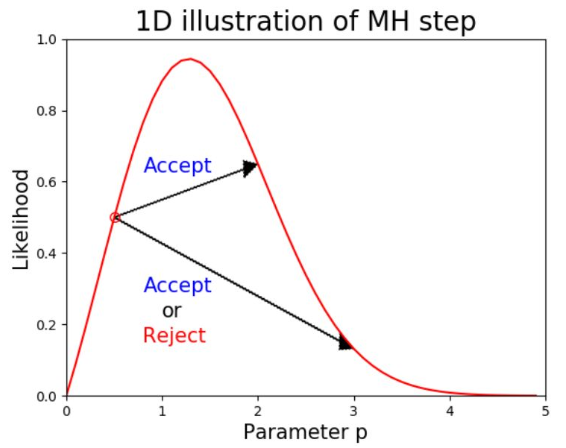
\includegraphics[width=\textwidth]{assets/MH_step.png}
    \captionof{figure}{Illustration of MH step}
    \label{fig:mcmc_efficiency}
\end{minipage}

\begin{warningblock}[Tuning and efficiency]
    Poorly chosen proposals lead to ineffective chains: very small steps yield high acceptance but slow random-walk exploration; very large steps produce tiny acceptance rates and correlated samples. Affine-invariant ensemble samplers (e.g.\ \textsc{emcee}) mitigate some tuning issues by evolving an ensemble of walkers.
\end{warningblock}

\subsubsection{Burn-in and convergence diagnostics}

The initial segment of a chain usually reflects the starting point more than the posterior. Standard practice is to discard a \textbf{burn-in} (or \textbf{warm-up}) phase until time-averaged statistics stabilize. There is no universal burn-in fraction; it depends on the proposal, parameterization, and data complexity.

Good MH chains look like white noise if you plot one parameters values throughout the chain

\begin{figure}[H]
    \centering
    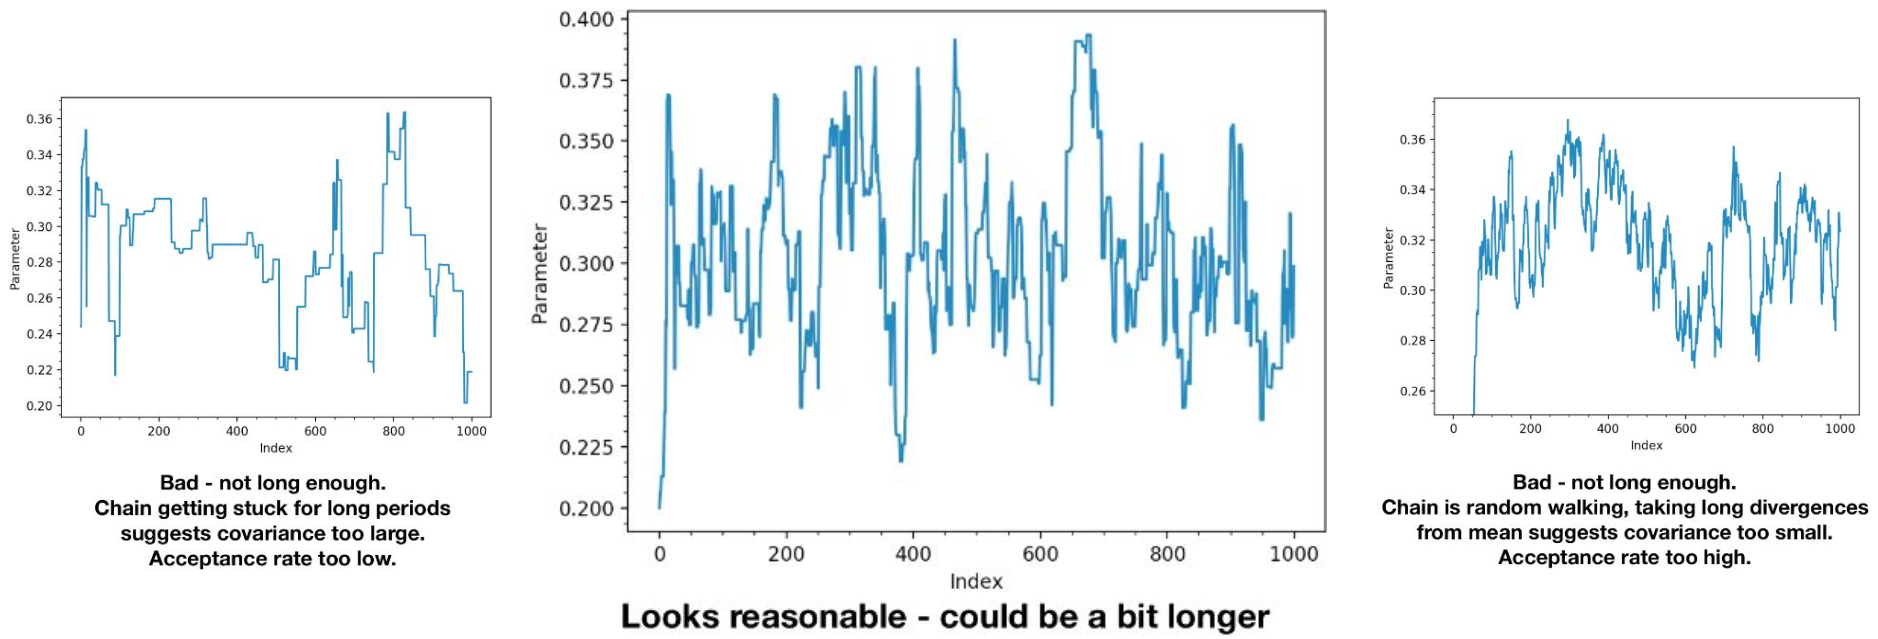
\includegraphics[width=0.9\textwidth]{assets/convergence.png}
    \caption{Example of MCMC chains converging after an initial burn-in phase.}
    \label{fig:burn_in}
\end{figure}

The \textbf{efficiency} of MCMC, and particularly Metropolis-Hastings, depends dramatically on how well the proposal distribution matches the shape and scale of the underlying posterior. A poorly chosen proposal may result in very slow convergence or failure to explore the relevant regions of parameter space. In practice, we rarely know the exact posterior geometry, but we can try to approximate it as closely as possible.

\subsection{Nested sampling}
\label{sec:nested_sampling}

Nested sampling targets the evidence directly while producing samples that can be post-processed into posterior draws. The key idea is to integrate the likelihood in slices of increasing contour $L > L_\star$, replacing high-dimensional volume integrals by one-dimensional sums over nested shells.

\begin{algorithm}[h]
    \caption{Sketch of nested sampling}
    \label{alg:NS}
    \begin{algorithmic}[1]
        \State Draw $N_{\mathrm{live}}$ points from the prior $\pi(\theta)$
        \While{stopping criterion on remaining evidence is not met}
            \State Find the point $\theta_i$ with smallest likelihood $L_i$
            \State Replace $\theta_i$ with a new point from the prior subject to $L(\theta) > L_i$
            \State Record the \textit{dead point} and its likelihood
        \EndWhile
        \State \textbf{Output:} posterior samples and accumulated evidence.
    \end{algorithmic}
\end{algorithm}

To get the posterior probability, simply histogram the parameter values vs weights.

\section{Goodness of fit}
\label{sec:goodness_of_fit}

\subsection{Chi-squared at the best fit}

The goodnes of fit is often estimated from the best-fit parameter values 
using a $\chi^2$ statistic (which is formally correct only for Gaussian 
distributed data) at the best-fit (or maximum-likelihood) parameters $\theta_{BF}$,
$$
\chi^2_{Best-fit} = (\vec d - \vec m (\theta_{BF}))^T C^{-1} (\vec d - \vec m (\theta_{BF}))
$$
where $\vec{d}$ is the data vector, $\vec{m}(\theta)$ the model prediction, and $\mathbf{C}$ the covariance matrix. This method does not account for the
uncertainties on the estimated parameters $\theta$.

\begin{tipsblock}[Uncertainties on data]
    \begin{minipage}{0.68\textwidth}
    When assessing the goodness of fit, it is essential to account for the uncertainties associated with the data.
    
    \medskip
    A small difference between the data and the model prediction does not necessarily indicate a good fit unless this discrepancy is understood relative to the measurement errors.
    \end{minipage}%
    \hfill
    \begin{minipage}{0.3\textwidth}
        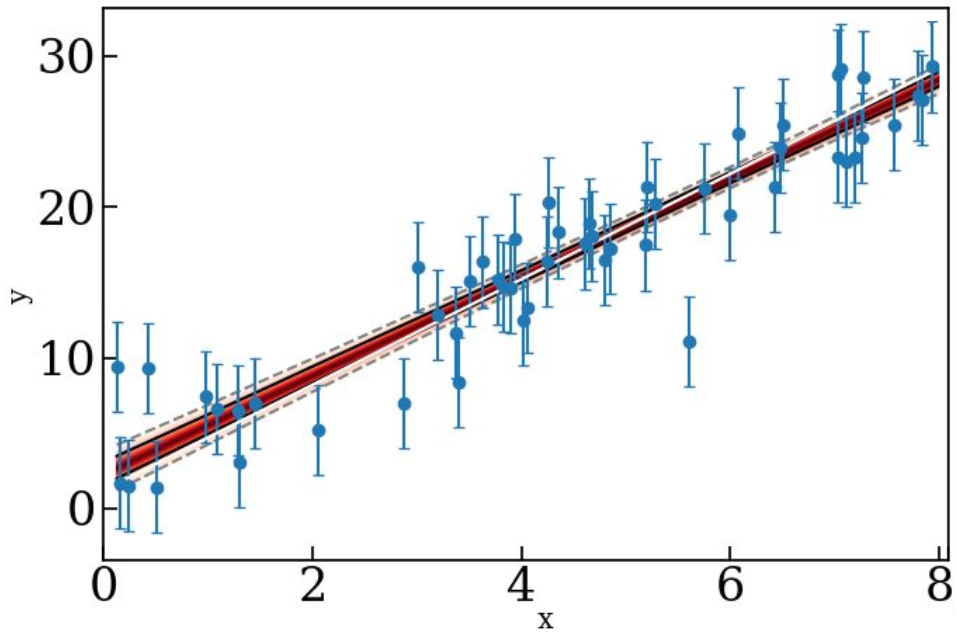
\includegraphics[width=\textwidth]{assets/model_fit.png}
    \end{minipage}
\end{tipsblock}

To assess the goodness of fit using $\chi^2_{Best-fit}$, one typically calculates the $p$-value $p(\chi^2 > \chi^2_{BF} | \nu)$, which represents the probability of obtaining a $\chi^2$ statistic larger than the observed $\chi^2_{BF}$ under the null hypothesis, assuming a $\chi^2$ distribution with $\nu$ degrees of freedom. Here, $\nu$ is often taken as the number of data points $N$ minus the number of model parameters.
However, in practice, the effective number of parameters may be less than the total number of free parameters, especially when parameters are correlated or subject to informative priors.

The reduced $\chi^2$ is defined as:
$$
\chi^2_{red} = \dfrac{\chi^2_{BF}}{\nu}
$$
It holds the following interpretation:
\begin{itemize}
    \item If $\chi^2_{red} \approx 1$, the model is a good fit for the data (residuals are of the same order as the uncertainties)
    \item If $\chi^2_{red} > 1$, the model might not fit well
    \item If $\chi^2_{red} \gg 1$, indicates systematic errors, underestimation of uncertainties, or a poor model
    \item If $\chi^2_{red} < 1$, The model may be overfitting or uncertaintites are overestimated
\end{itemize}

\subsection{Effective degrees of freedom from the posterior}

The effective number of constrained parameters can be quantified in several ways based on the posterior distribution. Common measures include:

\begin{align*}
N_{\Theta,\,\mathrm{var}} &= 2 \left[ \left\langle (\chi^2)^2 \right\rangle_{\Pr(\Theta|d)} - \left\langle \chi^2 \right\rangle_{\Pr(\Theta|d)}^2 \right] \\[1em]
N_{\Theta,\,\mathrm{like}} &= \left\langle \chi^2 \right\rangle_{\Pr(\Theta|d)} - \chi^2_{\min} \\[1em]
N_{\Theta,\,\mathrm{post}} &= \left\langle \chi^2 \right\rangle_{\Pr(\Theta|d)} - \chi^2 \big(\arg\max \Pr(\Theta|d)\big)
\end{align*}

where $\langle ... \rangle_{\Pr(\Theta|d)}$ denotes averaging over the posterior, $\chi^2_{\min}$ is the minimum value of $\chi^2$ in the sample, and $\arg\max \Pr(\Theta|d)$ denotes the parameter values of maximum posterior probability.

\subsubsection{Posterior Predictive Distribution}

A more rigorous and comprehensive way to assess the goodness of fit, that takes into account both the uncertainties in the data and uncertainties in the model parameters, is through the \textbf{Posterior Predictive Distribution} (PPD).

\begin{minipage}{0.52\textwidth}
The PPD gives the probability distribution for new or replicated data ($y^{rep}$), given the observed data ($y$). It is defined as:
$$
P(y^{rep}|y) = \int d\theta\;\underbrace{P(y^{rep}|\theta)}_{\text{Likelihood}}\,\overbrace{P(\theta|y)}^{\text{Posterior}}
$$
Here, $P(\theta|y)$ is the posterior probability distribution of the model parameters after observing the data, and $P(y^{rep}|\theta)$ gives the likelihood of seeing certain data values $y^{rep}$ if the parameters were $\theta$.
\end{minipage}%
\hfill
\begin{minipage}{0.45\textwidth}
    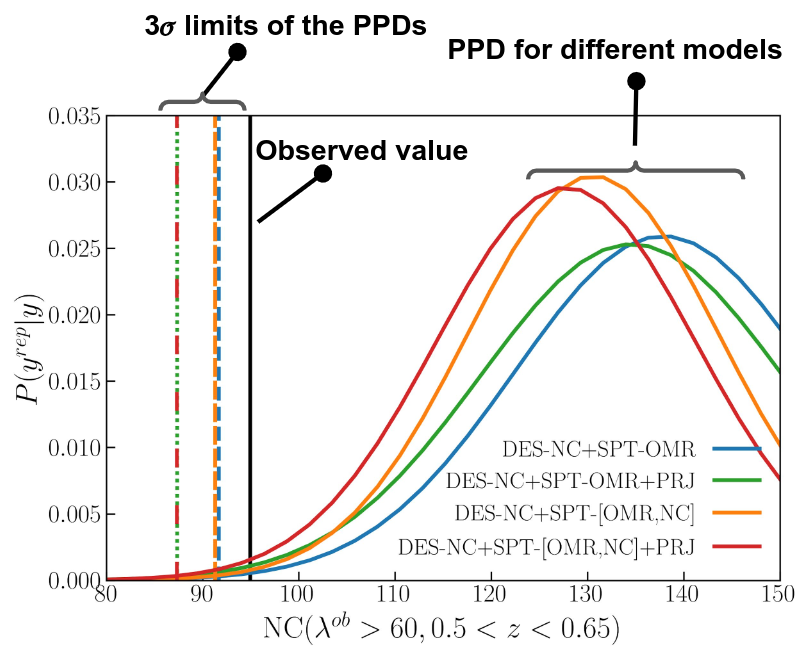
\includegraphics[width=0.9\textwidth]{assets/ppd.png}
    \captionof{figure}{PPD for the observed cluster count for 4 different model \cite{Costanzi_2021}}
    \label{fig:ppd}
\end{minipage}

The general procedure is as follows: 
\begin{enumerate}
    \item Draw values of $\theta$ from the posterior distribution $P(\theta|y)$ 
    (i.e., parameter samples that are plausible given the observed data).
    \item For each parameter $\theta$, generate a simulated (replicated) dataset $y^{rep}$ according to the model prediction $P(y^{rep}|\theta)$.
    \item Compare the ensemble of these mock datasets to the observed data $y$ to assess how typical the observed data appear under the model.
\end{enumerate}

To quantitatively evaluate the agreement between $y^{rep}$ and the observed data $y^{obs}$, one defines a test statistic $T(y, \theta)$, which is a function that can be computed for both the observed data and each mock realization. This statistic might, for example, measure the overall discrepancy between data and model (such as $\chi^2$), or highlight particular features of interest.

The \textbf{posterior predictive $p$-value} is then defined as:
$$
p = P(T(y^{rep}, \theta) > T(y^{obs}, \theta))
$$
This is the probability, over both the posterior and the distribution of replicated data, of obtaining a value of the test statistic greater than that observed. In other words, it measures how extreme the observed data are relative to what would typically be produced under the model and posterior.

A very low $p$-value (e.g., $p < 0.01$) means that the observed data are unlikely to have arisen if the model (and posterior) were correct, suggesting possible model misspecification. Conversely, a very high $p$-value (e.g., $p > 0.99$) can also indicate a problem (such as overfitting or an overestimated error budget). Ideally, a well-calibrated model produces $p$-values that are not systematically close to $0$ or $1$.

\medskip

The choice of test statistic $T$ is important and depends on the aspects of the fit one wishes to test. For high-dimensional datasets, especially with Gaussian-distributed errors, a common and useful choice is the $\chi^2$ statistic:
$$
T(d, \Theta) = (d-\mu(\Theta))^T C^{-1} (d-\mu(\Theta))
$$
where $d$ is the observed data vector, $\mu(\Theta)$ is the model prediction for parameters $\Theta$, and $C$ is the covariance matrix.

\subsection{Tension between data sets}

Assess the level of tension (or agreement) between posteriors derived from different data sets might not be trivial in a multi-dimensional parameter space.

\begin{exampleblock}[Tension between data sets]
    \begin{minipage}{0.68\textwidth}
    One-dimensional (1d) marginalized posteriors might appear to be in good agreement between different data sets, but this can be misleading: tensions may exist in the full multi-dimensional parameter space that are not visible in any 1d projection, a phenomenon known as ``projection effects''. In other words, two data sets could have 1d marginalized constraints that overlap for each parameter, yet still show significant inconsistency when analyzed jointly in more than one dimension.
    \end{minipage}%
    \hfill
    \begin{minipage}{0.3\textwidth}
        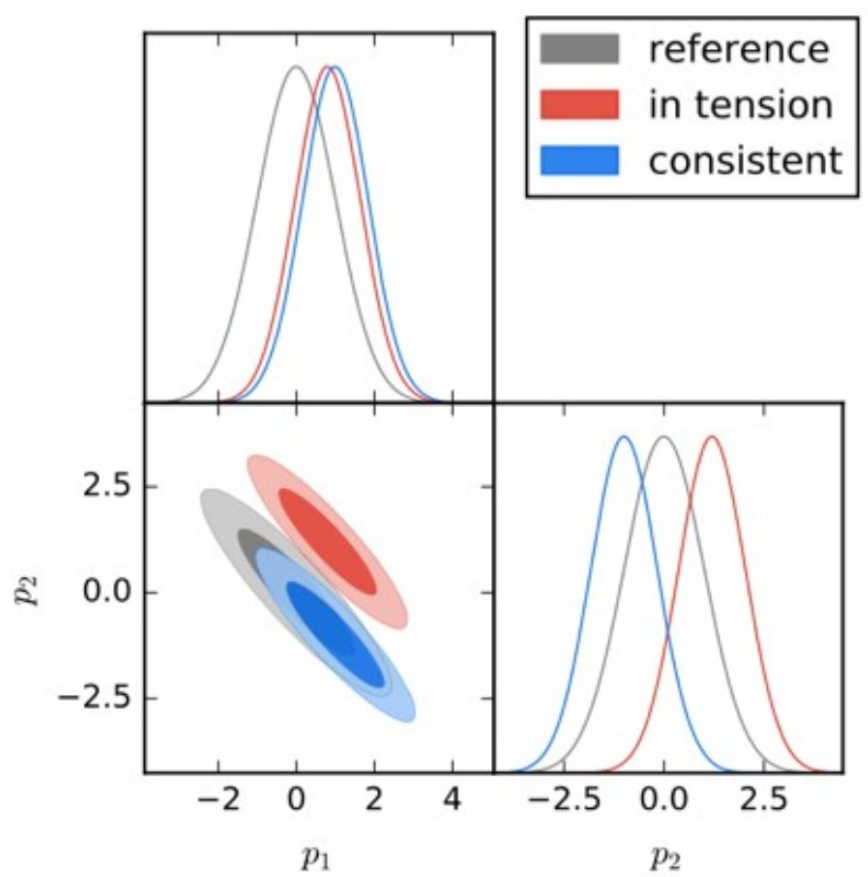
\includegraphics[width=0.98\textwidth]{assets/tension.png}
    \end{minipage}
\end{exampleblock}

There is no unique "metric" to assess the level of tension or agreement between data sets, and several approaches have been developed which can be broadly split into two categories:

\begin{itemize}
    \item \textbf{Evidence-based methods} :
    \emph{Given hypothesis $H_1$: ``The assumed model is capable of generating the data observed by both experiments'', and $H_2$: ``The assumed model is not capable of generating the data observed by both experiments'', which hypothesis is preferred by the data under the assumed model?} These methods require computing the \textbf{evidence}: $P(\vec{d}\,) = \int d\vec{\theta}\; \mathcal{L}(\vec{d}\,|\,\vec{\theta}) \pi(\vec{\theta})$
    \item \textbf{Parameter-space methods}: 
    \emph{What is the statistical significance of the differences between the posteriors for experiments $A$ and $B$, within the parameter space analyzed by both experiments?} \\
    These methods can often be computed directly from the parameter posteriors, but require good sampling of the tails of the distributions.
\end{itemize}

The tension between data sets can be quantified using the following \textbf{Tension Metrics}:

\begin{itemize}
    \item \textbf{Bayes Ratio}
    
    The Bayes Ratio $R$ is defined for infependent datasets $A$ and $B$  and for their combination $AB$ as:
    $$
    R \equiv \dfrac{\mathcal{Z}_{AB}}{\mathcal{Z}_{A}\mathcal{Z}_{B}}
    \qquad
    \text{where}
    \qquad
    \mathcal{Z}_{D} = P(D|M) = \int d\theta \mathcal{L}(D|\theta, M)\pi(\theta|M)
    $$
    In that expression, $\mathcal{Z}_{D}$ is the Bayesian Evidence, $\mathcal{L}$ is the likelihood of observing the data given model $M$ and parameter values $\theta$, and $\pi$ is the prior probability of those parameters given the model. $R$ can be viewed as a hypothesis test assessing the odds of both datasets being described with a single set of parameters ($\mathcal{Z}_{AB}$) as opposed to two independent sets of parameters ($\mathcal{Z}_{A}\mathcal{Z}_{B}$)

    Smaller values of $R$ indicate stronger evidence of tension between datasets $A$ and $B$.

    \item \textbf{Parameter difference technique}
    
    \begin{enumerate}
        \item Compute the parameter difference probability distribution:
        $$
            \mathcal{P}(\Delta\theta) = \int_{V_p} \mathcal{P}_A(\theta) \mathcal{P}_B(\theta - \Delta\theta)\, d\theta
        $$
        where $\mathcal{P}_A(\theta)$ and $\mathcal{P}_B(\theta)$ are the posterior distributions for parameter $\theta$ from experiments $A$ and $B$, respectively, and $\Delta\theta$ is the parameter difference.

        \item Determine the posterior mass above the iso-probability contour for no shift, i.e., $\Delta\theta = 0$:
        $$
            \Delta = \int_{\mathcal{P}(\Delta\theta) > \mathcal{P}(0)} \mathcal{P}(\Delta\theta)\, d\Delta\theta
        $$
   
        It gives the fraction of the posterior where the evidence for a shift exceeds that for no shift.
    \end{enumerate}
    
    This technique can be readily computed directly from the MCMC chains of experiments $A$ and $B$.

\end{itemize}

\subsection{Model Selection}

Model selection is the process of choosing the best model from a set of candidates. To determine which model is preferred by a given data set a simple comparison of $\chi^2$ might not be sufficient. Two widely used techniques are \bfit{Bayes Evidence Ratio} and \bfit{Deviance Information Criterion}.

\subsubsection{Bayes Evidence Ratio}

\vspace{-1em}

\begin{minipage}{0.58\textwidth}
The Bayes Evidence Ratio is defined as:
$$
\dfrac{P(M_1|\vec d)}{P(M_2|\vec d)} = \dfrac{P(\vec d|M_1)}{P(\vec d|M_2)} \dfrac{P(M_1)}{P(M_2)}
$$
The evidence is larger for a model if more of its parameter space is likely, and smaller for a model with large areas in its parameter space having low likelihood values, even if the likelihood function is sharply peaked.
\end{minipage}%
\hfill
\begin{minipage}{0.4\textwidth}
\begin{figure}[H]
    \centering
    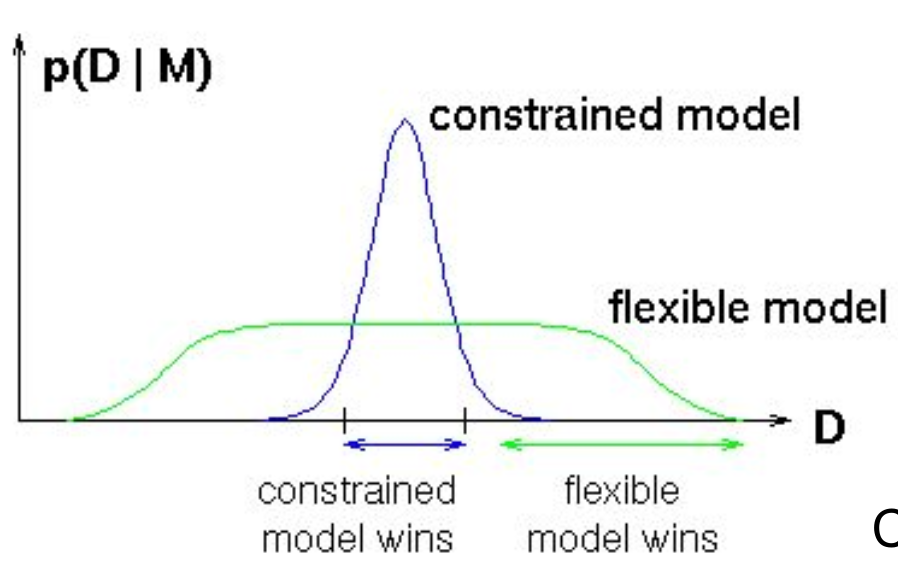
\includegraphics[width=\textwidth]{assets/model_selection.png}
\end{figure}
\end{minipage}

\subsubsection{Deviance Information Criterion}

The Deviance Information Criterion is defined as:
$$
DIC(M) = 2 \langle \chi^2 \rangle_M - \chi^2_{MaxP}(M)
$$
where:
\begin{itemize}
    \item $\langle \chi^2 \rangle_M$ is the mean $\chi^2$ posterior over the posterior volume
    \item $\chi^2_{MaxP}(M)$ is the $\chi^2$ at the maximum posterior point
\end{itemize}

The model with the lower DIC either fits better the data (lower $\langle \chi^2\rangle$) or has a lower level of complecity (lower $\langle \chi^2\rangle - \chi^2_{MaxP}$).

DIC can be easily computed directly from the parameters posteriors, but it is only strictly valid when the posterior distribution is well approximated by a multivariate Normal distribution.

\begin{exampleblock}[Prior dependence - DESI]
    \dots
\end{exampleblock}

\subsubsection{Prior Volume Effect}

The high-dimensionality of parameter spaces reduces the interpretability of posteriors to their one- and two-dimensional marginal distributions, when more information is available in the full dimensional distributions.

\begin{minipage}{0.55\textwidth}
Consider a scenario where the posterior is highly non-Gaussian and the true parameter values must be inferred. If we only have access to one-dimensional marginalized posteriors—for example, the six 1D projections in the illustration—it becomes challenging to accurately recover the true (fiducial) values using standard point estimators such as the best-fit, mean, or median. This is because, even if the full multi-dimensional posterior peaks at the correct parameters, marginalization over nuisance parameters can shift the apparent maxima in the reduced dimensions away from the truth. This systematic bias, inherent to the process of projection or marginalization in high-dimensional spaces, is known as the \textbf{prior volume effect} (or \textbf{projection effect}). It demonstrates how important information about parameter correlations and degeneracies can be lost during marginalization, potentially leading to misleading inferences if not properly accounted for.
\end{minipage}%
\hfill
\begin{minipage}{0.42\textwidth}
    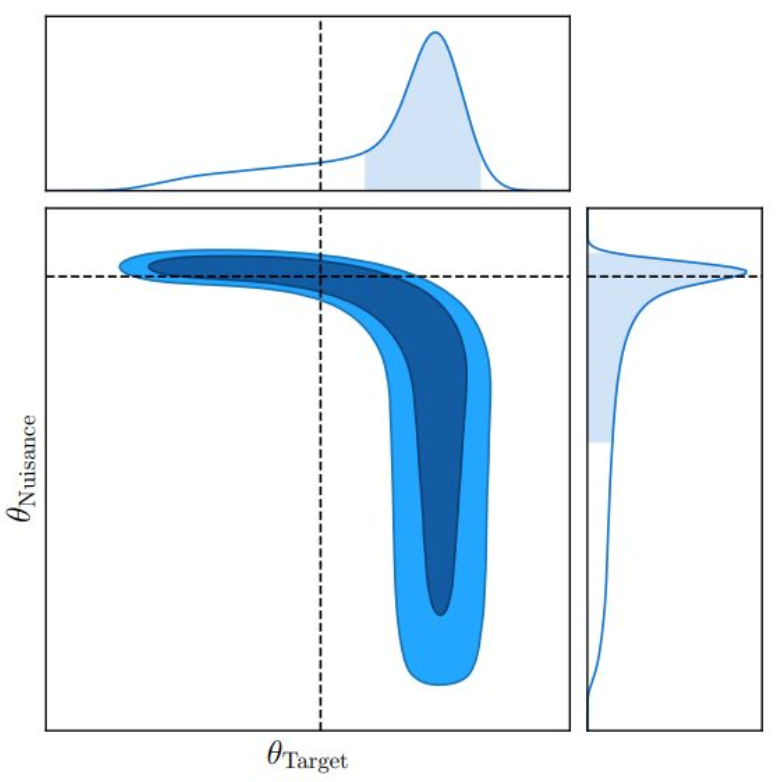
\includegraphics[width=\textwidth]{assets/prior_volume_effect.png}
    \captionof{figure}{Illustration of the prior volume (projection) effect: The true parameter value may be well-localized in the joint posterior, but its marginalized distributions can be shifted or broadened \cite{Ried_Guachalla_2025}.}
\end{minipage}

\begin{minipage}{0.35\textwidth}
    \centering
    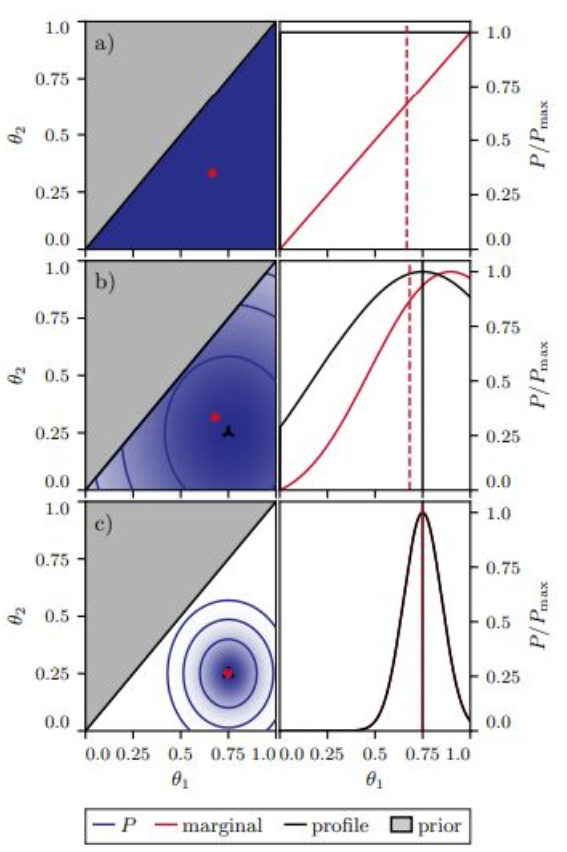
\includegraphics[width=\textwidth]{assets/prior_volume_effect_2.png}
\end{minipage}%
\hfill
\begin{minipage}{0.62\textwidth}
    \captionof{figure}{Difference between likelihood profiles and marginalized distributions, shown for increasingly constrained (narrower) posteriors. As the constraints tighten, projection effects diminish. \cite{Raveri_2024}.}

    \medskip

    Another manifestation of the prior volume effect arises when parameters are poorly constrained or highly prior-limited. In such cases, the marginalized posteriors can be significantly broadened or shifted due to projection over large and anisotropic volumes of parameter space.

    \medskip

    \noindent\textbf{Key insight:} \textit{Profile likelihoods} (or posterior profiles) are largely immune to projection effects since they maximize over nuisance parameters instead of integrating over them—they are sensitive only to the outline (shape) of the posterior, not to its total volume. An apt metaphor is that profiling traces the ridge-line of the posterior landscape, while marginalization is akin to summing the column density along each coordinate. Thus, profiling generally provides more robust parameter estimates in complex or high-dimensional models where marginalization may be misleading.
\end{minipage}